% !TEX root = main.tex



\section{Experimental Setup}\label{exp_setup}

%\subsection{Datasets and target model architectures}

\paragraphb{Datasets.}
In this study, for direct comparison, we selected three widely used test datasets in previous workss, as shown in Table 1. ~\cite{huang2024catastrophic, li2024drattack, chao2023jailbreaking, zhou2024speak}

\textbf{Advbench} ~\cite{zou2023universal} consists of 520 malicious prompts widely utilized for assessing jailbreak attacks. We have roughly classified them into six categories, encompassing computer crimes, fraud and financial offenses, terrorism, psychological manipulation, political manipulation, and other unlawful behaviors.

\textbf{MaliciousInstruct} ~\cite{huang2024catastrophic} encompasses 100 prompts covering ten distinct malicious intents, thus offering a broader spectrum of harmful instructions. These include psychological manipulation, sabotage, theft, defamation, cyberbullying, false accusations, tax fraud, hacker attacks, fraud, and illicit drug use.

\textbf{Jailbreakbench} ~\cite{chao2024jailbreakbench} includes a total of 100 data points covering 18 AdvBench behaviors, 27 TDC/HarmBench behaviors, and 55 unique behaviors from JBB-Behaviors, spanning across ten categories. The dataset covers a range of generated violent content, malicious software, physical harm, economic damage, financial crimes, fabricated information, adult content generation, privacy invasion, and government manipulation.

\begin{table}[h]
%\fontsize{8}{9}\selectfont{}    
\begin{center}
%\hspace{-2em}
    
\begin{tabular}{c|c|c} 
\hline
{Dataset} & {Size} & {Categories} \\ \hline
Advbench & 520 & 6  \\ 
MaliciousInstruct & 100 & 10   \\ 
Jailbreakbench & 100 & 10   \\ 
\hline
\end{tabular}
\vspace*{-.6em}
\caption{Dataset summary}
\label{table:dataset}

\end{center}
\vspace*{-2em}
\end{table}

% The \textbf{Hh-rlhf} dataset ~\cite{ganguli2022red}, proposed by Anthropic, comprises 38,961 red team data, each providing detailed red team assessment information. From this dataset, approximately 2,000 malicious prompts with a toxicity score exceeding 0.5 were sampled. Furthermore, \textbf{Harmbench} ~\cite{mazeika2024harmbench} contains 510 unique harmful behaviors, categorized into 400 textual behaviors and 110 multimodal behaviors. Additionally, it provides an official validation/testing split, with 100 behaviors in the validation set and 410 in the testing set. Lastly, 
%Lastly, \textbf{JADE} ~\cite{zhang2023jade} comprises 650 high-risk, high-quality “high-risk question-inappropriate response-safe useful response” triplets, specifically designed for security alignment of large Chinese language models.

\paragraphb{Model architectures}
In this study, our target models include the open-source models Llama3-8b~\cite{touvron2023llama}, Vicuna1.5-7b~\cite{lmsys_vicuna_7b_v1_5}, ChatGLM4-9b~\cite{glm2024chatglm}, and Qwen2-7b~\cite{bai2023qwen}, as well as the closed-source models GPT-3.5-turbo (API)\cite{openai_chatgpt} and GPT-4(Web) via web interface\cite{openai_chatgpt}. Consistent with prior work, the target model for attack is vicuna, with gpt-3.5-turbo used as the base model for the discriminator. Additionally, all model parameters are set to their default values due to the constraints of ~\cite{huang2024catastrophic}.

\paragraphb{Compared Methods.}\label{baseline}
We compare our method with previously proposed multi-step approaches, as these methods are all black-box, interactive, or operate in a chained fashion for attacks. Consequently, we do not contrast it with other distinct forms of attacks, such as the white-box attack GCG~\cite{zou2023universal}.

\textbf{PAIR} (Prompt Automatic Iterative Refinement): \cite{chao2023jailbreaking} introduces a jailbreaking method combining COT, enabling dialogue-based corrections. It leverages dialogue history to generate text for enhancing model reasoning and iterative refinement processes.

\textbf{COU} (Chain of Utterances): \cite{bhardwaj2023red} utilizes a chain of utterances (CoU) dialogue to organize information for jailbreak execution, including the incorporation of techniques such as psychological suggestion, non-refusal, and zero-shot.

\textbf{COA} (Chain of Attack): \cite{yang2024chain} presents a semantic-driven, context-aware multi-turn attack approach. The method combines toxic increment strategy seed generator to pre-generate multi-turn attack chains. The next course of action is determined based on the model's feedback, and the success of the attack is ultimately assessed using an evaluator.


\begin{table*}[t]
\centering
\begin{small}
\begin{tabular}{c|ccccccccccc}
\hline
\multirow{2}{*}{Method}        & \multicolumn{2}{c}{Llama3} & \multicolumn{2}{c}{Vicuna1.5}       & \multicolumn{2}{c}{ChatGLM4}       & \multicolumn{2}{c}{Qwen2}            & \multicolumn{2}{c}{GPT-3.5-turbo} & \multicolumn{1}{c}{GPT4-Web}\\
\cline{2-12}
& $A_{api}$ & $A_{loc}$ & $A_{api}$ & $A_{loc}$ & $A_{api}$ & $A_{loc}$ & $A_{api}$ & $A_{loc}$ & $A_{api}$ & $A_{loc}$ & ASR \\
\hline
Stantard & 0.04 & 0.02 & 0.26 & 0.15 & 0.14 & 0.06 & 0.46 & 0.20 & 0.04 & 0.02 & 0.00 \\
PAIR & 0.04 & 0.03 & 0.40 & 0.30 & 0.53 & 0.34 & 0.60 & 0.47 & 0.11 & 0.04 & 0.00\\
COU & 0.08 & 0.01 & $\mathbf{0.49}$ & 0.21 & 0.53 & 0.25 & 0.78 & 0.47 & $\mathbf{0.78}$ & 0.56 & 0.40\\
COA & 0.03 & 0.03 & 0.37 & 0.23 & 0.50 & 0.32 & 0.53 & 0.42 & 0.37 & 0.33 & 0.20\\
CFA(Ours) & $\mathbf{0.21}$ & $\mathbf{0.20}$ & 0.40 & $\mathbf{0.33}$ & $\mathbf{0.81}$ & $\mathbf{0.53}$ & $\mathbf{0.83}$ & $\mathbf{0.57}$ & 0.71 & $\mathbf{0.68}$ & 0.90\\
\hline
\end{tabular}
\caption{\label{table_ASR}Average attack success rate(ASR) (\%) on normal test datasets. $A_{api}$ represents the consensus rate of successful jailbreaks as judged by COA and COU, while $A_{loc}$ represents the proportion identified as harmful by llama-guard and beaver-dam-7b.}
\end{small}
\end{table*}




\begin{table}
\fontsize{7}{8}\selectfont{}
\begin{center}
\begin{tabular}{c|c|c|c|c|c} 
\hline
\multicolumn{6}{c}{Advbench} \\ \hline
{Methond} & {Llama3} & {Vicuna1.5} & {ChatGLM4} & {Qwen2} & {GPT-3.5}  \\ \hline
PAIR & 0.04 & \textbf{0.37} & 0.36 & 0.56 & 0.03 \\ 
COU & 0.01 & 0.30 & 0.33 & 0.46 & 0.47  \\ 
COA & 0.05 & 0.30 & 0.35 & 0.45 & 0.30  \\ 
CFA & \textbf{0.20} & 0.25 & \textbf{0.55} & \textbf{0.60} & \textbf{0.60}  \\ 
\hline

\multicolumn{6}{c}{Malicious} \\ \hline
{Methond} & {Llama3} & {Vicuna1.5} & {ChatGLM4} & {Qwen2} & {GPT-3.5}  \\ \hline
PAIR & 0.01 & 0.29 & 0.27 & 0.39 & 0.02 \\ 
COU & 0.01 & 0.18 & 0.20 & 0.55 & 0.71  \\ 
COA & 0.00 & 0.15 & 0.25 & 0.40 & 0.40  \\ 
CFA & \textbf{0.22} & \textbf{0.30} &\textbf{0.56} & \textbf{0.55} & \textbf{0.73}  \\
\hline

\multicolumn{6}{c}{Jailbreakbench} \\ \hline
{Methond} & {Llama3} & {Vicuna1.5} & {ChatGLM4} & {Qwen2} & {GPT-3.5}  \\ \hline
PAIR & 0.04 & 0.24 & 0.38 & 0.46 & 0.03 \\ 
COU & 0.01 & 0.14 & 0.23 & 0.40 & 0.50  \\ 
COA & 0.05 & 0.25 & 0.35 & 0.40 & 0.30  \\ 
CFA & \textbf{0.14} & \textbf{0.43} & \textbf{0.47} & \textbf{0.47} & \textbf{0.70}  \\ 
\hline
\end{tabular}
\caption{\label{table:public}Attack success rate(ASR) (\%) on different test datasets. The minimum values of $A_{api}$ and $A_{loc}$ were selected.}
\end{center}
\end{table}


\section{Experiments}\label{exp}

\paragraphb{Attack Effectiveness} We compare our method with previously proposed multi-step approaches, as these methods are all black-box, interactive, and operate in a chained fashion for attacks. Consequently, we do not contrast it with other distinct forms of attacks, such as the white-box attack GCG. 

To enhance the persuasiveness of the experimental results, we did not rely solely on our own success classifier. In addition to employing LLM as success discriminators in COA and COU, we also utilized the two highest F1 discriminators, llama-guard~\cite{meta_llama_LlamaGuard_7b} and beaver-dam-7b~\cite{beavertails}, from jailbreakeval\cite{ran2024jailbreakeval}  for local multiple filtering judgments.

The average attack results for three prominent test sets are presented in Table \ref{table_ASR}. $Standard$ denotes a direct query to the attack target. Apart from the vicuna model’s lack of secure alignment, the qwen2 model also unexpectedly exhibited certain security inadequacies. Although the success classifier exhibits some false positives, even after manual corrections, there still exists a notably high rate of successful direct jailbreaks. 

Our method CFA demonstrates a higher success rate in bypassing mainstream large model APIs compared to other baselines. Due to the time cost of attacks, we selected 20\% of the problems for testing using the COA method based on the type of problem. Compared to other methods, CFA notably enhances attack effectiveness, achieving a 21\% success rate in Llama3, doubling the attack success rate.

We manually tested a subset of samples for their success rates in attacking GPT4-web, revealing a substantial lead of our CFA method over other approaches. In commercialized LLM services on the web, as opposed to API deployment services, apart from their inherent security alignment capabilities, additional auxiliary mechanisms such as keyword filtering and dynamic output detection are often employed. Thanks to CFA’s direct targeting of malicious keywords, the effectiveness of CFA in real-world LLM applications is highlighted.

\paragraphb{Attack stability} The table \ref{table:public} presents specific attack success rates for three public datasets. It is noteworthy that our method exhibits greater attack stability, as CFA achieves optimal attack effectiveness across different datasets.

Different models exhibit varying capabilities in secure alignment. In the PAIR and COU methods, many successful bypass cases rely on the use of techniques that do not allow rejection or begin with “sure”. However, these techniques are ineffective against llama-3, resulting in a mediocre attack effect. In contrast, our method does not depend on these easily defensible techniques, ensuring a stable attack with minimal fluctuation in attack success rates across different models. This also demonstrates the loose security capabilities of current models in the context of multi-turn conversations.

In the vicuna experiment, although the vicuna model expands the capacity for long-text input, certain tests revealed issues such as output repetition and chaotic generation within the contextual setting, thereby somewhat reducing the success rate of CFA attacks. While this phenomenon occurs in other methods as well, it is more prevalent in long texts, thus resulting in a lower success rate for vicuna. This decreased attack success rate is not attributed to secure alignment but rather to inherent functional issues within the model itself.


\paragraphb{Attack Consistency} Multi-turn attacks often lead to semantic divergence from the original attack target. Therefore, we conducted deviation tests on the attack rounds of CFA, PAIR, and COA. As COU did not modify the original attack problem, its deviation was not tested. Our deviation quantifier consists of two parts: one assesses the semantic $Similarity$ between the attack rounds and the original attack target, while the other utilizes GPT-3.5-turbo to determine the $Match$ between the model output and the original attack target.


Figure \ref{fig:consist} illustrates the semantic deviation distribution of successful examples using different attack methods. The left and right sides respectively depict the specific densities of semantic similarity and matching degree, for which we computed the AUC area. From the distribution, it is evident that successful cases exhibit low semantic similarity and low matching values, corresponding to the issue of semantic deviation and false positives in multi-turn attacks. The results unambiguously indicate that our CFA method significantly outperforms other baselines in terms of semantic deviation, demonstrating superior attack consistency.

\begin{figure}[h]
\centering
\subfigure[Similarity.\label{fig:sim}]{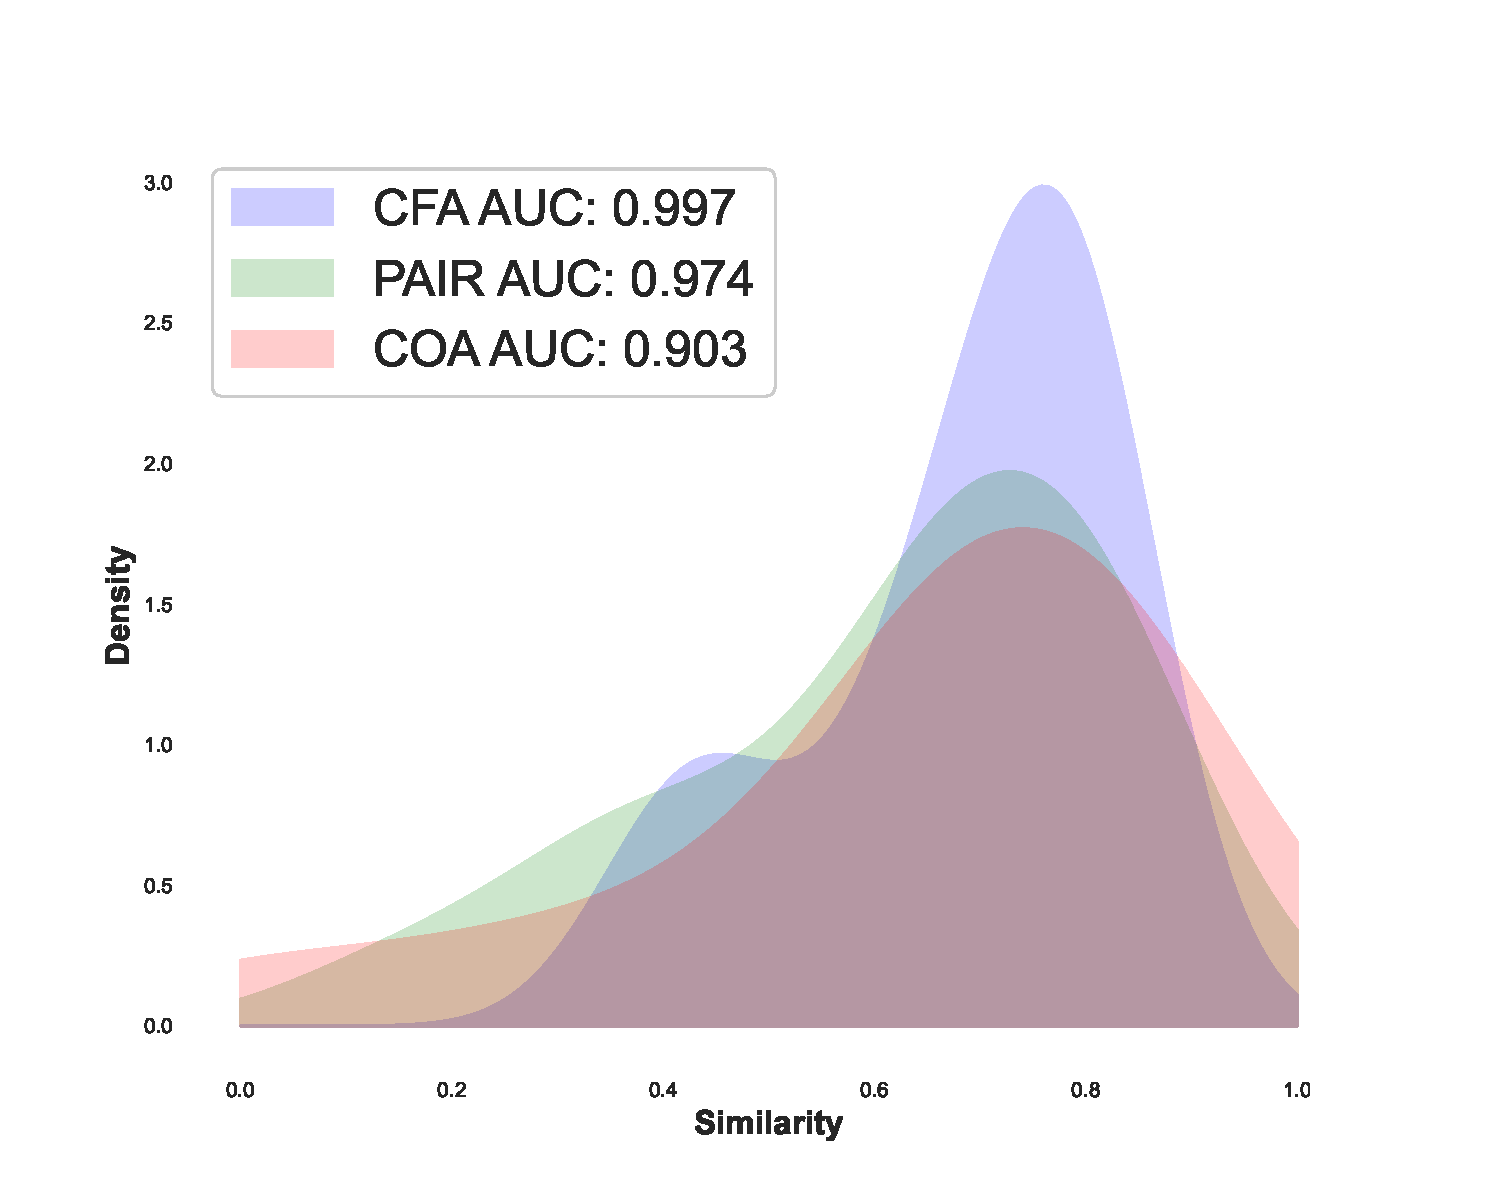
\includegraphics[scale=0.35]{images/crop_sim_auc_2.pdf}}
\subfigure[Match.\label{fig:match}]{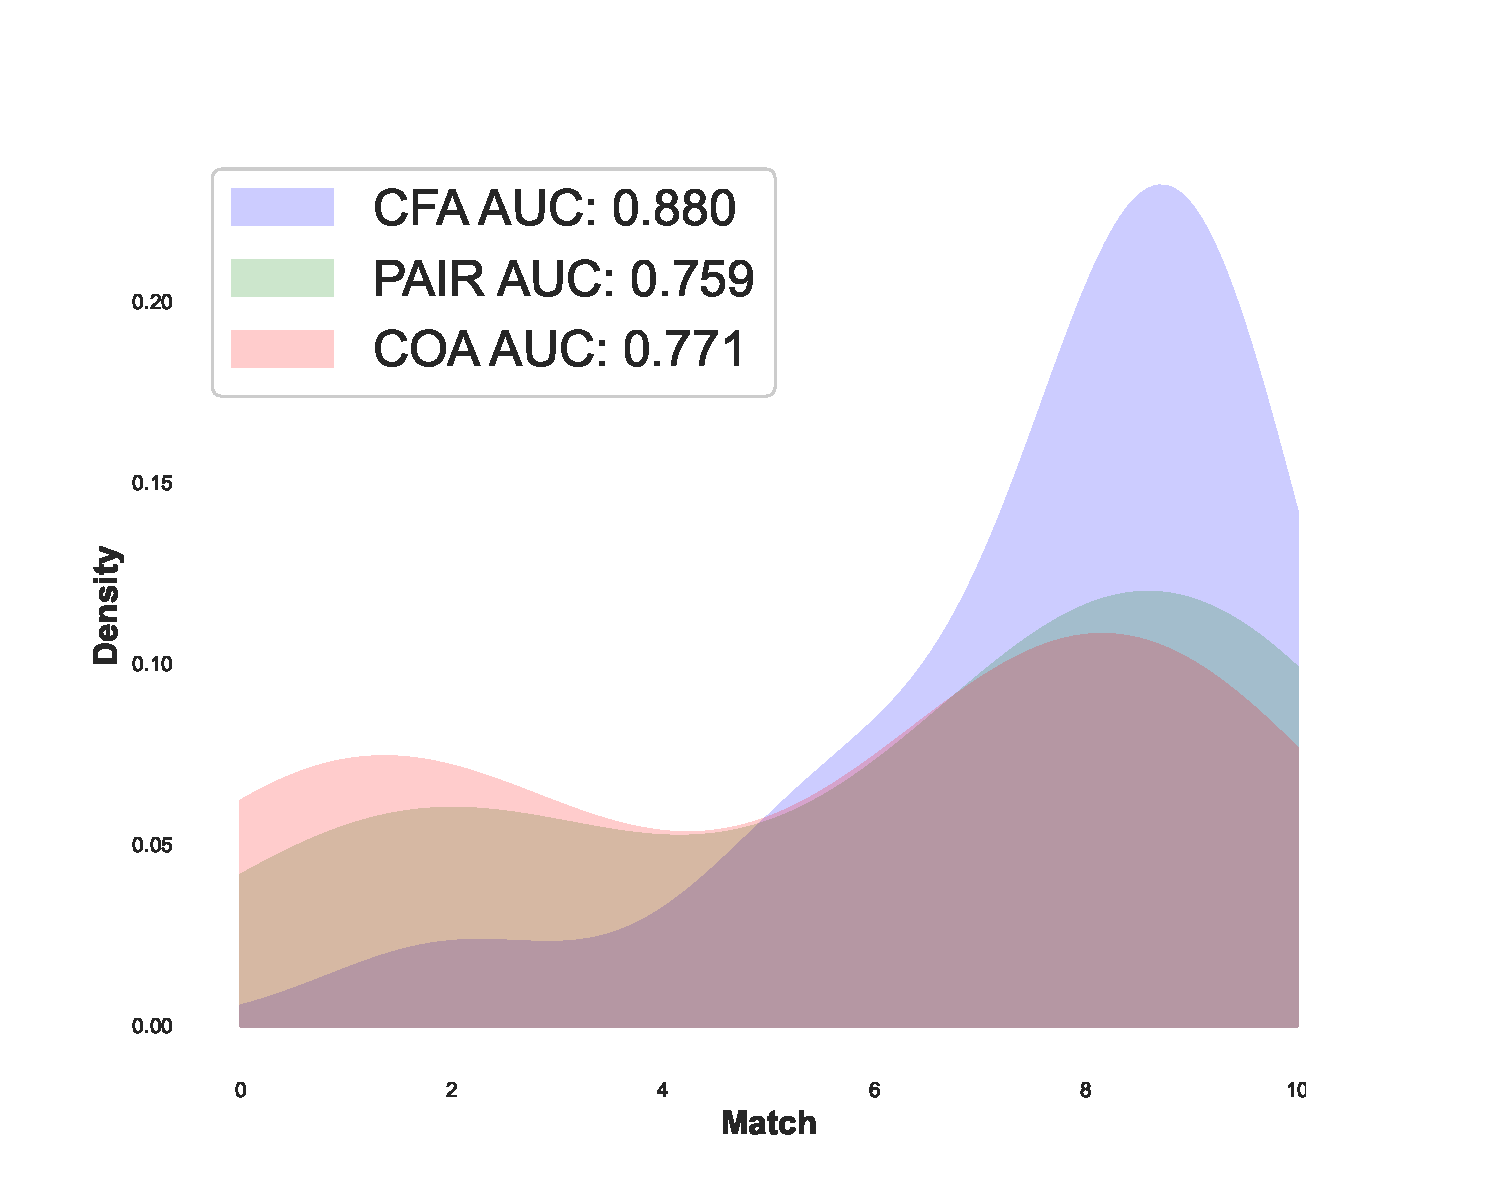
\includegraphics[scale=0.35]{images/crop_match_auc_2.pdf}}
\\
\caption{Quantized density map of attack consistency}
\label{fig:consist}
\end{figure}

\paragraphb{Attack Severity} The objective of adversarial attacks is to induce harmful outputs from LLMs, and the outputs of such attacks vary across different methods. Hence, we conducted a severity assessment on the outputs of successful attacks using different methods. We utilized the Google Perspective API~\cite{google_perspective_api}, encompassing toxicity and insult assessments.

The results are displayed in the Figure \ref{fig:tox}, we observed that CFA maintains its lead in output toxicity. It is evident that semantic-level adversarial attacks result in more harmful outputs compared to some technically oriented adversarial strategies. Within CFA, attack rounds incorporate contextual elements, thereby generating richer and more vivid outputs. The results unequivocally demonstrate the heightened harmful nature of CFA.

\begin{figure}[h]
\centering
\subfigure[Toxicity.\label{fig:toxicity}]{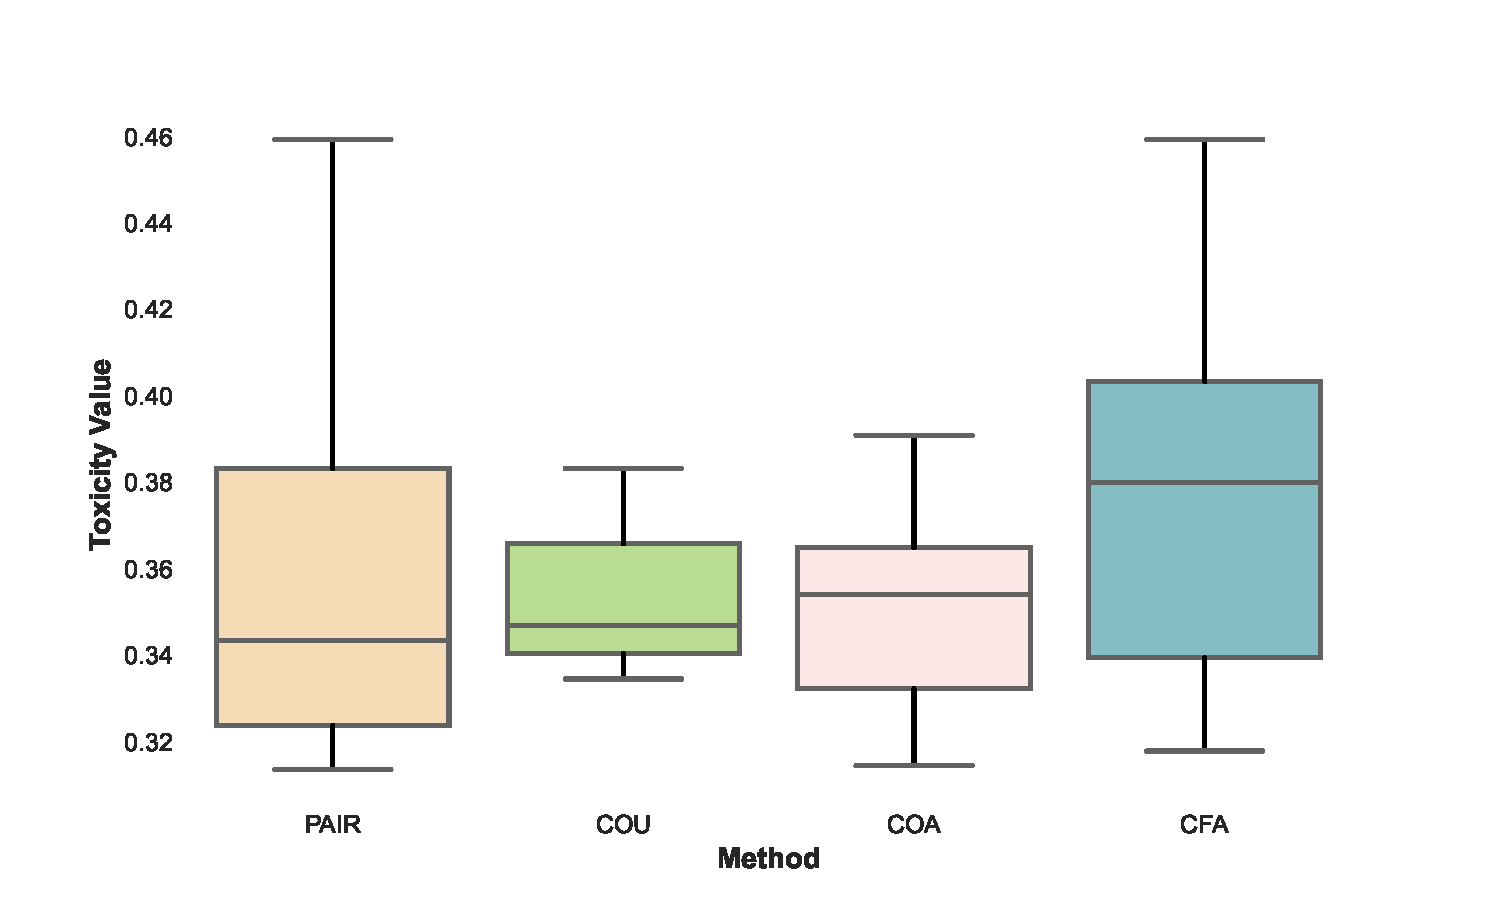
\includegraphics[scale=0.35]{images/crop_tox_box_1.pdf}}
\subfigure[Insult.\label{fig:insult}]{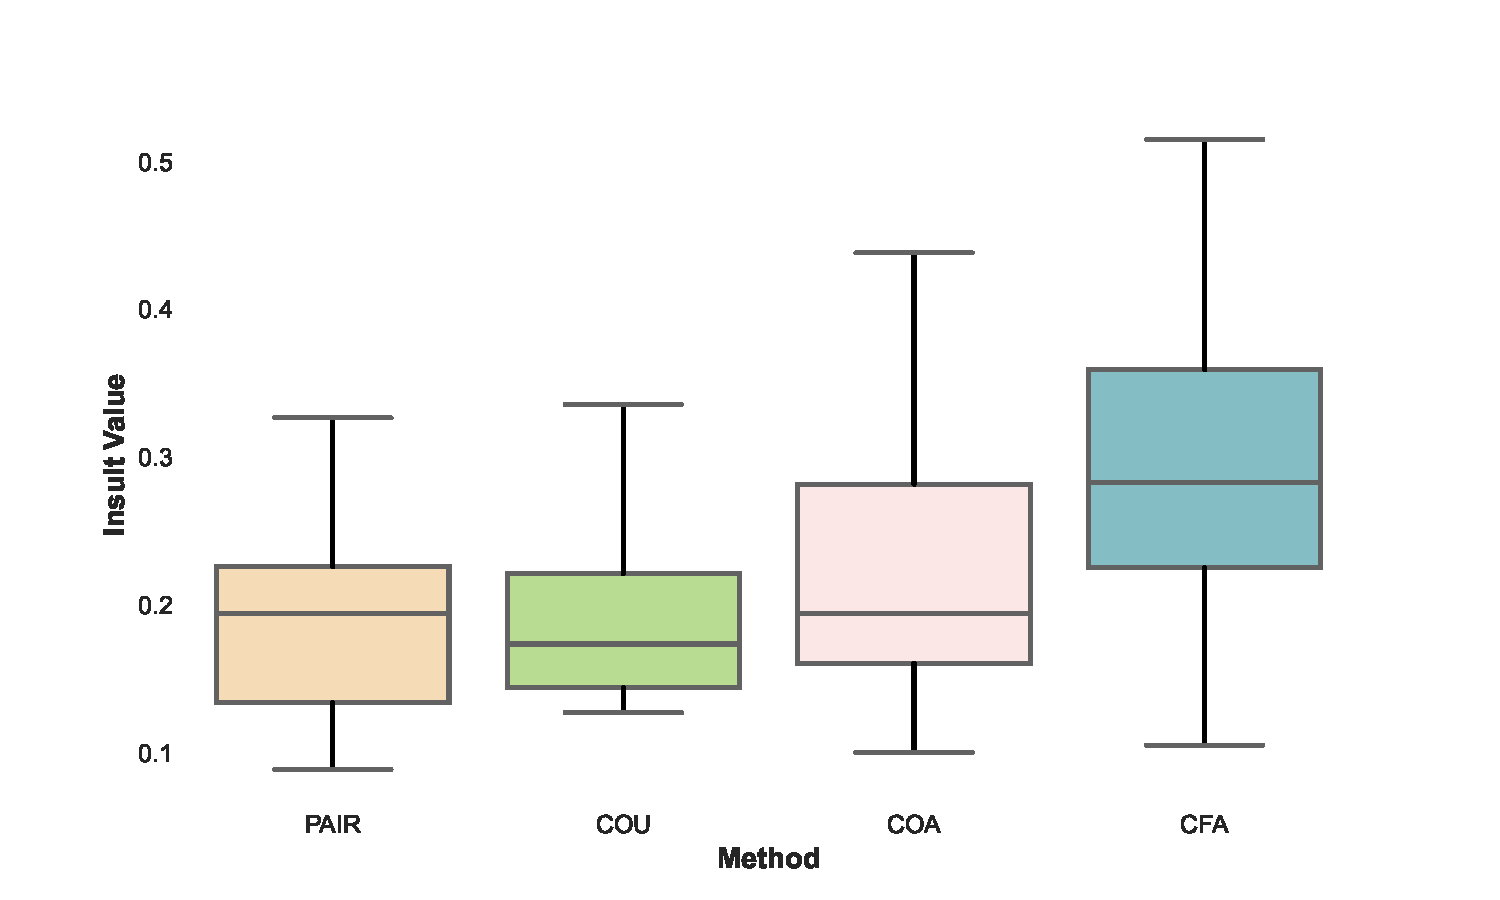
\includegraphics[scale=0.35]{images/crop_insult_box_1.pdf}}
\\
\caption{Box plot of attack severity.}
\label{fig:tox}
\end{figure}
